\section{Methods}

\subsection{Method overview}

This work compares the outcomes of patients under two treatment delivery models: i) \emph{usual care}, in which the patient is taken to their nearest emergency hospital for IVT, and for patients with with onwards transfer to a MT-capable centre for patients considered likely to eligible for MT (which involves additional travel time and other transfer-related delays); ii) \textit{MSU care}, in which an MSU attends the patient on-scene to provide IVT, with patients with an LVO (shown on an on-scene CT angiogram) being taken directly to their most local MT-capable centre. The scope of the modelling includes the stroke patients’ pathway from stroke onset to treatment with IVT and, where appropriate, MT, with this time to treatment being translated to the patient outcome, which is dependent also on the stroke type and treatment received. Strokes are defined as either an nLVO or LVO, with their treatment options being IVT (for an nLVO) or IVT followed by MT (for an LVO). We explore sensitivities around pathway process durations using scenario analysis, the variation due to the stroke onset location using geographic analysis, and the impact of the number of MSU base locations on patient outcomes. It was assumed throughout that there were no resource restrictions upon the use of MSUs, with complete implementation across all areas, and that all eligible patients with an LVO would receive MT. The maxiumum time from stroke onset to receiving treatment was 4.5 hours for IVT, and 8 hours for MT - configurations of MT base locations may be chosen such that for some patients treatment would not be possible due to process times exceeding these treatment time thresholds.

Our modelling compares outcomes for those patients receiving IVT or MT. We do not make any assumption about the proportion of all patients receiving those treatments.

\subsection{Lower Super Output Areas (LSOA)}

We performed our analysis across England using LSOA as our geographic footprint \cite{ons}. LSOAs are small areas in England, with roughly 1,500 people in each area (they were designed for demographic data collection, with each area having roughly the same number of people, rather than being the same geographic size). There are 32,843 LSOAs in England.

\subsection{Stroke admission data}

Stroke admission numbers per LSOA were taken from Hospital Episode Statistics (HES) 2017-2019 (using ICD-10 codes of I61, I63 and I64). Across those three years, in total there were 242,874 recorded stroke admissions coming from an England LSOA going to one of the 101 acute stroke units in England (an average of 2.47 admissions per LSOA per year). The stroke patient population were divided into stroke type cohorts, based on vessel occlusion type (LVO and nLVO). Using analysis from reperfusion treatment clinical trials \cite{lees_time_2010, emberson_effect_2014, goyal_endovascular_2016, fransen_time_2016}, we classify each patient's vessel occlusion type based on their National Institutes of Health Stroke Scale (NIHSS) on arrival (NIHSS 0-10 as nLVO; NIHSS 11+ as LVO), as NIHSS has been shown to have higher accuracy in separating nLVO and LVO than other stroke scales (Area Under the Receiver Operating Characteristic Curve = 0.86 \cite{duvekot_comparison_2021}). Applying this classification to the stroke admission data in England and Wales (Sentinel Stroke National Audit Programme), this provides an estimate of 30\% LVO and 70\% nLVO in the treatable population. This proportion split was applied to each of the LSOAs in the study (to divide the total stroke admissions by LSOA as provided by HES into these two patient stroke type cohorts). These derived values were also cross-checked against stroke types identified in studies on pre-hospital selection of patients with suspected LVO \cite{de_la_ossa_herrero_design_2013}, where LVO made up 38\% of the population where a pre-hospital diagnostic (RACE score) was applied. Population density was taken from the Office of National Statistics 2011 census.

\subsection{Pathway processes modelling}

All code used for usual care and MSU care pathway modelling is available \cite{github1}.

Figure \ref{fig:process} describes the processes included in the three pathways that are modelled: two pathways for usual care depending on which type of stroke centre is nearest to the LSOA, and one pathway for MSU care. \textit{Usual care} is provided by the patient attending their nearest stroke centre, which is either i) a \textit{primary stroke centre}, PSC, providing IVT only, with onward transfer for LVO patients  requiring MT to the comprehensive stroke centre that is nearest to the PSC, or ii) a \textit{comprehensive stroke centre}, CSC, providing both IVT and MT. The \textit{MSU care} pathway involves the MSU providing on-scene IVT, followed by the MSU transferring the LVO patients to the closest CSC for MT. The onwards transfer of nLVO patients is not included in the scope of this modelling.

Based on input from three co-production workshops \cite{moseley_co-design_2024} involving representation from stroke consultants, ambulance staff and patients and public (4-6 from each group at each of three workshops), we designed the model to explore large numbers of possible parameter values (see \emph{scenario analysis} section for more detail). This reflected the uncertainty of how the MSUs would operate and perform if implemented.

Unless specified otherwise, it was assumed that MSUs are located at CSCs. We also assume MSUs are equipped with CT angiography (CTA) and can identify LVO patients who will benefit from direct transfer to a CSC for MT.

Geographic analysis was undertaken at LSOA level. Travel times from each of the 32,843 LSOAs in England to all hospitals (PSC and CSCs), and travel times between hospitals have been estimated using Open Street Map data, with results calibrated against Google Maps. Travel times have been made available \cite{gitlab1}.

\begin{figure}[h]
    \centering
    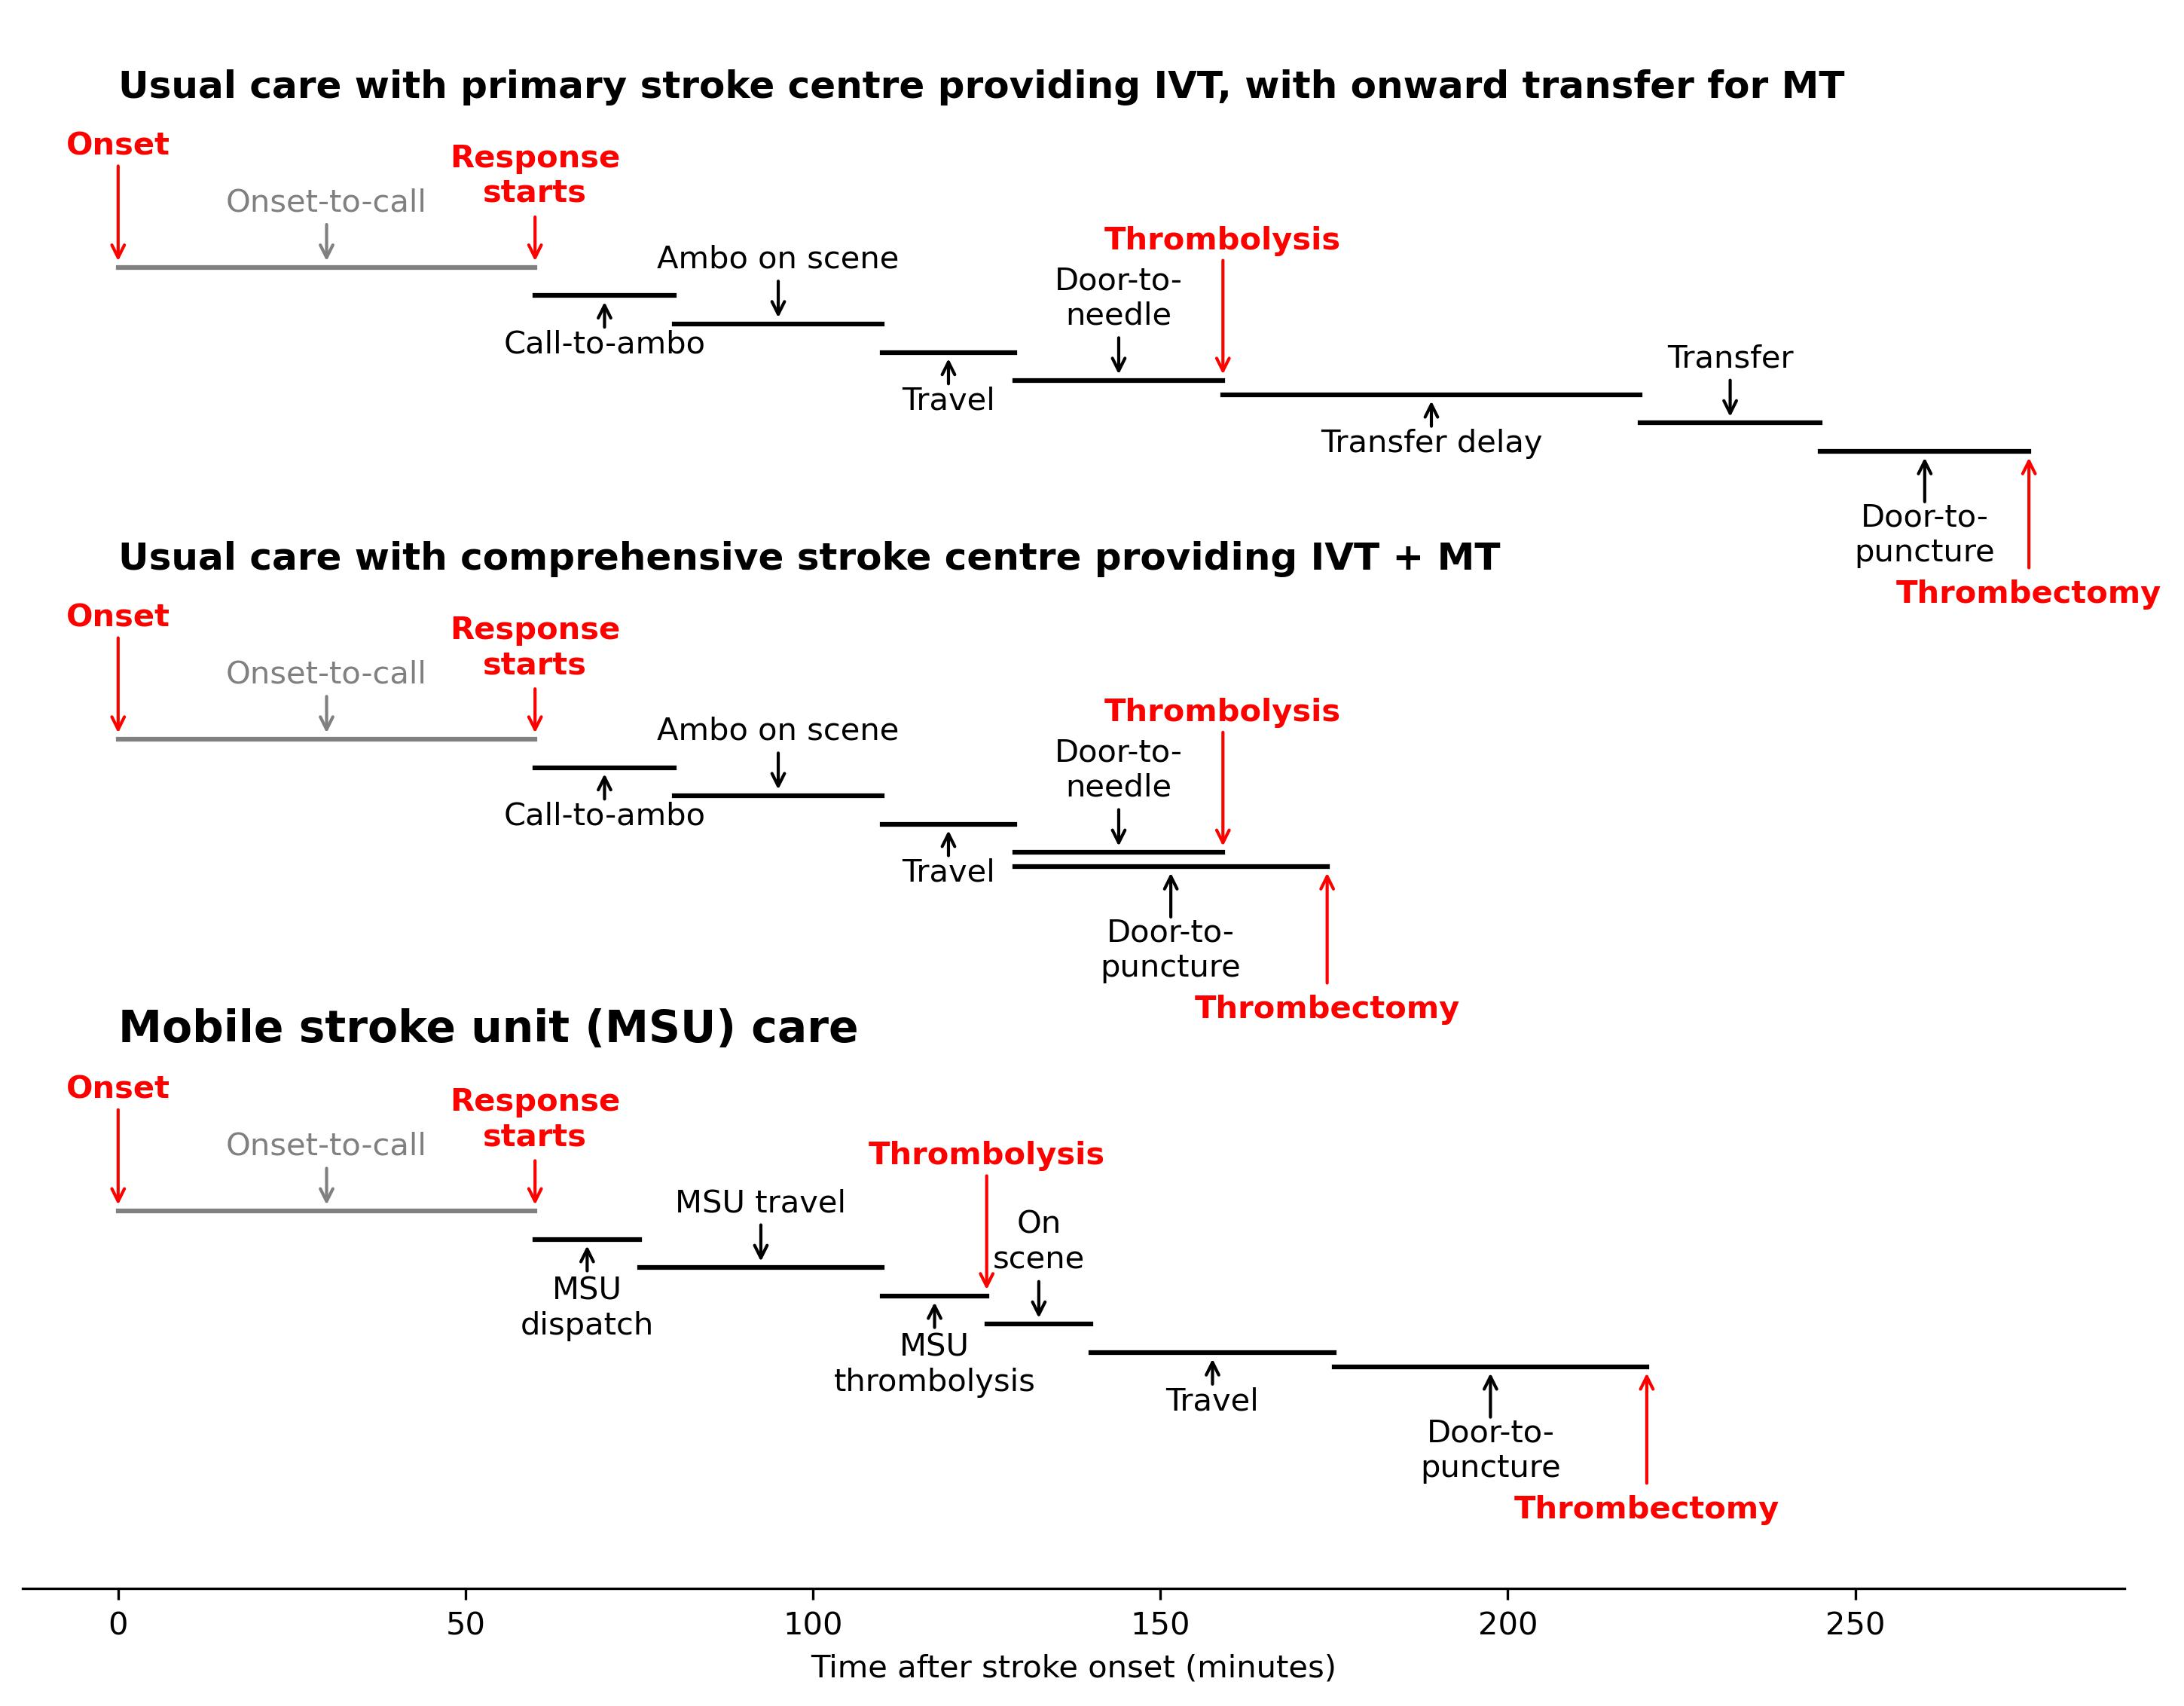
\includegraphics[width=0.85\linewidth]{images/stroke_treatment.jpg}
    \caption{An illustrative timeline showing processes included in the three pathways that are modelled for provision of IVT and MT. Top: Usual care pathway for patients with a PSC closest to their home LSOA, with the PSC providing IVT, followed by the LVO patients having a transfer to the nearest CSC for MT. Middle: Usual care pathway for patients with a CSC closest to their home LSOA, with the CSC providing both IVT and MT. Bottom: MSU care pathway, with IVT provided on-scene by the MSU, followed by the MSU transferring the LVO patients to the nearest CSC for MT. Process times other than travel times are common for all patients (defined by the scenario). Travel times depend on locations of patient and hospitals, with results calculated for all LSOAs in England. n.b. ``ambo'' is short for ``ambulance''.}
    \label{fig:process}
\end{figure}

For each LSOA, times to IVT and MT are calculated by summing all the non-travel process times (common for all patients and defined by the scenario) and adding required travel times (bespoke for each LSOA location, and for each inter-hospital transfer). The next section will describe how patient outcomes are calculated based on these LSOA-specific times to IVT and MT for usual care or MSU care. All calculations are performed in Python/NumPy.

\subsection{Outcome modelling}

Outcome modelling is based on published meta-analysis of clinical trials which have evaluated the decline of effectiveness  of IVT and MT over time \cite{emberson_effect_2014, fransen_time_2016}. We have applied those models to the expected real world treatment population (based on the national stroke audit of England and Wales, SSNAP). We report the expected benefit in the treated population (using a mix of nLVO and LVO derived from the patients currently arriving at hospital within 4 hours of stroke onset - as this is likely to be similar to the population where a MSU is dispatched and IVT treatment is given on-scene). 

Detailed methods and code used for modelling these outcomes are available \cite{github2}, with methods described in the appendix and as an online book \cite{github3}. The outcome model is available as a PyPI package for Python \cite{pypi}.

We used modified Rankin Scale (mRS) at 3--6 months as a measure of outcome. mRS is the most commonly used instrument to describe post-stroke functional outcome \cite{quinn_functional_2009}, describing independence of living from a scale of 0 (no disability) through to 5 (severe disability requiring constant nursing attention), with death assigned an mRS of 6. A commonly used surrogate for independent living is mRS 0--2. Health utility values for each mRS level were taken from Wang \textit{et al.} \cite{wang_utility-weighted_2020}. The mean mRS score, mean utility and proportion of patients with mRS 0--2 in a given mRS distribution can be compared between scenarios.

We calculated the patients' mRS outcome distribution based on time to treatment for three patient-treatment cohorts: nLVO treated with IVT; LVO treated with IVT alone; and LVO treated with IVT and MT. For each patient-treatment cohort we calculated an mRS distribution for treatment at any given time by interpolating between the mRS distribution for treatment given at \emph{t=0} (time of stroke onset) and the mRS distribution for treatment given at \emph{t=No Effect} (time of no effect of treatment), assuming that log odds fall linearly over time \cite{emberson_effect_2014, fransen_time_2016}. Further details on how these \emph{t=0} and \emph{t=No Effect} mRS distributions were derived are given in the supplementary material.

The time to no effect was 6.3 hours for IVT \cite{emberson_effect_2014} and 8.0 hours for MT \cite{ fransen_time_2016}. Our model did not include selection of patients who may still benefit from treatment beyond these durations through the use of perfusion scanning. This number is small for IVT, but is more substantial for MT – approximately 2500 per annum in England. 

\subsection{Scenario analysis}

Scenario analysis was undertaken to investigate how changing assumed model parameters (the process durations, in minutes) affect outcomes across all LSOAs. The parameter values were varied according to the following, with all combinations modelled:

\vspace{5mm}

\begin{minipage}{1.0\textwidth}  % Define the width of the minipage
\begin{itemize}
    \item All patients:
    \begin{itemize}
        \item Stroke onset to call: 0, 60, 120, 180
    \end{itemize}
    \item Usual care:
    \begin{itemize}
        \item Call to ambulance arrival: 15, 30, 45
        \item Ambulance on-scene: 20, 30, 45
        \item Hospital arrival to IVT (door-to-needle): 30, 45
        \item Transfer-related net MT delay (excluding travel time): 30, 60, 90
        \item Hospital arrival to MT (door-to-puncture): 60, 90, 120
    \end{itemize}
    \item Mobile stroke units:
    \begin{itemize}
        \item Call to MSU dispatch: 0, 15, 30, 45
        \item MSU arrival to IVT: 15, 30, 45
        \item MSU on-scene post-IVT: 5, 15
        \item MSU hospital arrival to MT (door-to-puncture): 30, 60, 90
    \end{itemize}
\end{itemize}
\end{minipage}

\vspace{5mm}

At the CSC in the usual care pathway, the \emph{hospital arrival to MT} time has been shown to be shorter for patients transferred from a PSC than for patients who are directly admitted \cite{hassan_impact_2022}. This is due to some of the necessary processes (such as information gathering, imaging and IVT) already being completed at the PSC. However, these patients will experience a delay in receiving MT (in addition to their inter-hospital travel time) due to waiting for transfer from the PSC. These two time durations (additional time waiting for transfer and shorter \emph{hospital arrival to MT}) are represented in the model as a single parameter: the \emph{transfer-related net MT delay} parameter. For example, if the time spent in the PSC is 90 minutes (known as the \textit{door-in-door-out} time), but the \textit{hospital arrival to MT} is reduced by 30 minutes, this is represented by setting \textit{transfer-related net MT delay} to 60 minutes in the model and leaving the \emph{hospital arrival to MT} unchanged.

\subsection{Geographic analysis}

To study geographic variation in benefit of MSU care, a single set of parameters was chosen that reflected a reasonable base case for performance of usual care and MSU care. Process times (minutes) are shown in the following list, with ambulance and MSU travel times and inter-hospital travel times dependent on patient location (LSOA). In this base case scenario MSUs are based at CSCs only. 

\vspace{5mm}

\begin{minipage}{1.0\textwidth}  % Define the width of the minipage
\begin{itemize}
    \item All patients:
    \begin{itemize}
        \item Stroke onset to call: 60
    \end{itemize}
    \item Usual care:
    \begin{itemize}
        \item Call to ambulance arrival: 20
        \item Ambulance on-scene: 30
        \item Hospital arrival to IVT: 45
        \item Transfer-related net MT delay (excluding travel time): 60
        \item Hospital arrival to MT: 90
    \end{itemize}
    \item Mobile stroke units:
    \begin{itemize}
        \item Call to MSU dispatch: 15
        \item MSU arrival to IVT: 30
        \item MSU on-scene post-IVT: 5
        \item MSU hospital arrival to MT: 60
    \end{itemize}
\end{itemize}
\end{minipage}

\vspace{5mm}

\subsection{Varying number of MSU base locations}

In order to study the effect of changing the number of MSU base locations, a greedy algorithm was used. In this method, 100 MSU base locations are sequentially added, with each additional one chosen from the 101 current acute stroke units (of any type, CSC or not), in the order of maximum improvement in outcomes (utility). The utility gain is calculated for those patients treated by an MSU rather than usual care; the algorithm is therefore looking at the effect of changing the number of MSU base locations, rather than the number of MSU vehicles. The algorithm can also be run with MSU base locations chosen from only the 23 current CSCs.